\documentclass[12pt,a4paper]{article}

\usepackage[margin=1in]{geometry}
\usepackage{amsmath, amssymb, amsthm}
\usepackage{enumitem}
\usepackage{tikz}
\usetikzlibrary{arrows.meta, positioning}

\setlength{\parindent}{0pt}
\setlength{\parskip}{6pt}

\newtheoremstyle{notestyle}
  {8pt}
  {8pt}
  {\normalfont}
  {}
  {\bfseries}
  {.}
  {0.5em}
  {}

\theoremstyle{notestyle}
\newtheorem{definition}{Definition}
\newtheorem{example}{Example}

\newenvironment{answer}
{\par\textbf{Answer.}\ }
{\hfill$\square$\par}

\newcommand{\Prob}{\mathbb{P}}

\title{\textbf{Supplementary Notes: Fair Gambler's Chain}}
\author{MA4034: Time Series and Stochastic Processes}
\date{}

\begin{document}
\maketitle

\section{What is the Fair Gambler's Chain?}

The fair gambler's chain is a Markov chain that describes the fortune of a gambler who repeatedly plays a fair game.

Suppose the gambler's fortune after $n$ games is
\[
X_n.
\]

The state space is
\[
S=\{0,1,2,3,\ldots\}.
\]

Here:
\begin{itemize}[leftmargin=1.2cm]
    \item state $0$ means the gambler has no money,
    \item state $1$ means the gambler has 1 dollar,
    \item state $2$ means the gambler has 2 dollars,
    \item and so on.
\end{itemize}

The game is called \textbf{fair} because the probability of winning 1 dollar is equal to the probability of losing 1 dollar:
\[
\Prob(\text{win})=\frac12,
\qquad
\Prob(\text{lose})=\frac12.
\]

So from state $i\geq 1$:
\[
i\to i+1
\quad\text{with probability }\frac12,
\]
and
\[
i\to i-1
\quad\text{with probability }\frac12.
\]

\section{Why is State 0 Special?}

In the version used in the lecture, state $0$ is not absorbing. Instead, when the gambler is at state $0$, they can either:
\begin{itemize}[leftmargin=1.2cm]
    \item stay at $0$ with probability $\frac12$,
    \item move to $1$ with probability $\frac12$.
\end{itemize}

One way to understand this is: if the gambler becomes broke, someone gives them another dollar to continue playing, but there is still a possibility of staying at zero for one step.

Thus,
\[
0\to 0
\quad\text{with probability }\frac12,
\]
and
\[
0\to 1
\quad\text{with probability }\frac12.
\]

\section{Transition Diagram}

\begin{center}
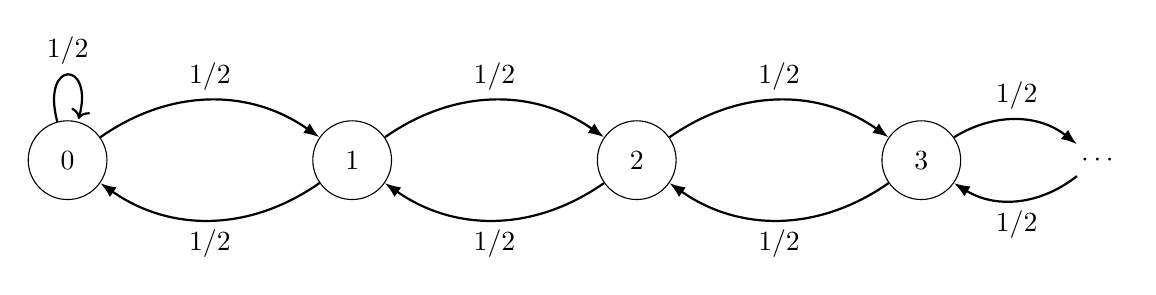
\begin{tikzpicture}[
  state/.style={circle, draw, minimum size=10mm},
  edge/.style={-{Latex[length=2mm]}, thick},
  bend angle=35
]
\node[state] (0) {$0$};
\node[state, right=26mm of 0] (1) {$1$};
\node[state, right=26mm of 1] (2) {$2$};
\node[state, right=26mm of 2] (3) {$3$};
\node[right=14mm of 3] (dots) {$\cdots$};

\draw[edge] (0) edge[loop above] node {$1/2$} (0);
\draw[edge] (0) edge[bend left] node[above] {$1/2$} (1);
\draw[edge] (1) edge[bend left] node[below] {$1/2$} (0);
\draw[edge] (1) edge[bend left] node[above] {$1/2$} (2);
\draw[edge] (2) edge[bend left] node[below] {$1/2$} (1);
\draw[edge] (2) edge[bend left] node[above] {$1/2$} (3);
\draw[edge] (3) edge[bend left] node[below] {$1/2$} (2);
\draw[edge] (3) edge[bend left] node[above] {$1/2$} (dots);
\draw[edge] (dots) edge[bend left] node[below] {$1/2$} (3);
\end{tikzpicture}
\end{center}

\section{Transition Matrix}

Using the state order
\[
0,1,2,3,\ldots,
\]
the transition matrix is
\[
P=
\begin{pmatrix}
\frac12 & \frac12 & 0 & 0 & 0 & \cdots\\
\frac12 & 0 & \frac12 & 0 & 0 & \cdots\\
0 & \frac12 & 0 & \frac12 & 0 & \cdots\\
0 & 0 & \frac12 & 0 & \frac12 & \cdots\\
\vdots & \vdots & \vdots & \vdots & \vdots & \ddots
\end{pmatrix}.
\]

\subsection{How to Read the Matrix}

The rows represent the current state. The columns represent the next state.

For example, the first row is
\[
\left(\frac12,\frac12,0,0,\ldots\right).
\]
This means that from state $0$:
\[
p_{00}=\frac12,
\qquad
p_{01}=\frac12.
\]

The second row is
\[
\left(\frac12,0,\frac12,0,\ldots\right).
\]
This means that from state $1$:
\[
p_{10}=\frac12,
\qquad
p_{12}=\frac12.
\]

The third row is
\[
\left(0,\frac12,0,\frac12,\ldots\right).
\]
This means that from state $2$:
\[
p_{21}=\frac12,
\qquad
p_{23}=\frac12.
\]

\section{Why is it a Markov Chain?}

The next fortune depends only on the current fortune.

For example, if the gambler currently has 5 dollars, then the next fortune is:
\[
6 \quad\text{with probability }\frac12,
\]
or
\[
4 \quad\text{with probability }\frac12.
\]

It does not matter how the gambler reached 5 dollars. Therefore the process has the Markov property.

\section{Worked Example}

\begin{example}
Suppose the gambler starts with 2 dollars. Find the probability that after one game the gambler has 3 dollars. Also find the probability that after one game the gambler has 1 dollar.
\end{example}

\begin{answer}
Starting from state $2$, the gambler can move to:
\[
3
\quad\text{with probability }\frac12,
\]
or
\[
1
\quad\text{with probability }\frac12.
\]

Therefore,
\[
\Prob(X_1=3\mid X_0=2)=\frac12,
\]
and
\[
\Prob(X_1=1\mid X_0=2)=\frac12.
\]
\end{answer}

\begin{example}
Suppose the gambler starts with 1 dollar. Find the probability that after two games the gambler has 1 dollar again.
\end{example}

\begin{answer}
Starting from state $1$, the gambler can return to state $1$ after two games in two ways:
\[
1\to 0\to 1,
\]
or
\[
1\to 2\to 1.
\]

The probability of the first path is
\[
\frac12\cdot\frac12=\frac14.
\]

The probability of the second path is
\[
\frac12\cdot\frac12=\frac14.
\]

Therefore,
\[
\Prob(X_2=1\mid X_0=1)
=
\frac14+\frac14
=
\frac12.
\]

Thus,
\[
\boxed{p_{11}^{(2)}=\frac12.}
\]
\end{answer}

\section{Practice Questions}

\begin{enumerate}[label=\textbf{Q\arabic*.}, leftmargin=1.2cm]
    \item What does state $4$ mean in the fair gambler's chain?

    \item If the gambler is currently at state $5$, what are the possible next states and their probabilities?

    \item If the gambler is currently at state $0$, what are the possible next states and their probabilities?

    \item Write the row of the transition matrix corresponding to state $3$.

    \item Starting from state $2$, find the probability of being at state $2$ after two steps.

    \item Starting from state $0$, find the probability of being at state $0$ after two steps.

    \item Is the fair gambler's chain irreducible? Explain.

    \item Why is it called fair?
\end{enumerate}

\section{Answers}

\subsection*{Answer 1}

State $4$ means the gambler currently has 4 dollars.

\[
\boxed{X_n=4\text{ means the fortune after }n\text{ games is 4 dollars.}}
\]

\subsection*{Answer 2}

From state $5$, the gambler can win 1 dollar or lose 1 dollar.

Therefore:
\[
5\to 6
\quad\text{with probability }\frac12,
\]
and
\[
5\to 4
\quad\text{with probability }\frac12.
\]

\subsection*{Answer 3}

From state $0$, in this version of the fair gambler's chain:
\[
0\to 0
\quad\text{with probability }\frac12,
\]
and
\[
0\to 1
\quad\text{with probability }\frac12.
\]

\subsection*{Answer 4}

From state $3$:
\[
3\to 2
\quad\text{with probability }\frac12,
\]
and
\[
3\to 4
\quad\text{with probability }\frac12.
\]

Therefore the row corresponding to state $3$ is
\[
(0,0,\frac12,0,\frac12,0,\ldots).
\]

\subsection*{Answer 5}

Starting from state $2$, to return to state $2$ after two steps, there are two possible paths:
\[
2\to 1\to 2,
\]
and
\[
2\to 3\to 2.
\]

The first path has probability
\[
\frac12\cdot\frac12=\frac14.
\]

The second path has probability
\[
\frac12\cdot\frac12=\frac14.
\]

Therefore,
\[
\Prob(X_2=2\mid X_0=2)
=
\frac14+\frac14
=
\frac12.
\]

\subsection*{Answer 6}

Starting from state $0$, to be at state $0$ after two steps, there are two possible paths:
\[
0\to 0\to 0,
\]
and
\[
0\to 1\to 0.
\]

The first path has probability
\[
\frac12\cdot\frac12=\frac14.
\]

The second path has probability
\[
\frac12\cdot\frac12=\frac14.
\]

Therefore,
\[
\Prob(X_2=0\mid X_0=0)
=
\frac14+\frac14
=
\frac12.
\]

\subsection*{Answer 7}

Yes, the fair gambler's chain is irreducible.

From any state $i$, the chain can move down step by step until it reaches state $0$. Also, from state $0$, the chain can move up step by step to reach any state $j$.

Thus, for any states $i$ and $j$,
\[
i\to j
\]
is possible.

Therefore all states communicate, and the chain is irreducible.

\[
\boxed{\text{Irreducible}}
\]

\subsection*{Answer 8}

It is called fair because the probability of winning 1 dollar is equal to the probability of losing 1 dollar:
\[
\Prob(\text{win})=\frac12,
\qquad
\Prob(\text{lose})=\frac12.
\]

There is no advantage toward winning or losing in a single step.

\end{document}
